\chapter{DESIGN DETAILS AND IMPLEMENTATION}
To implement a low cost IoT application which can be help full for industrial application. The components we have used for our objective and major requirements are explained in this part.Implementation of the objective, software and hardware requirement are taken as an overview in this chapter.

\section{REQUIREMENT ANALYSIS}
\subsection {Software Requirements}
Arduino IDE ,python IDE, Raspbien OS. 
 \subsection{Hardware Requirements}
Ultrasonic sensor, sound sensor, vibration sensor, smoke sensor, humidity and temperature sensor, two Arduino boards, raspberry pi, breadboard, connecting wires, two Bluetooth modules and wifi module.  



\section{Component details}
Major components that are involved in achieving our objective are as below;
\subsection{Sound sensor }  Working voltage: Dc 4 ~ 6v has the signal output instructions single signal and responds output. Effective signal output for low level. 

\subsection{Ultrasonic sensor} Supply voltage- 5 v, global current consumption -15 A, ultrasonic frequency -40k Hz, maximal range -400 cm, minimal range-minimal range- 3 cm, resolution -1 cm, trigger pulse width -10 us , outline dimension- 43x20x15 mm.

\subsection{SM-420 Vibration sensor }
Supply- voltage 3.3 to 5 v, On-board LED indicator to show the results, switch default state is close, On-board LM393 chip. 

\subsection{MQ-2 Smoke sensor }
Operating voltage is +5 v, the voltage of analog output is 0-5 v and the voltage of digital output is 0-5 v. Preheat duration will be 20 seconds. It can be used as analog and digital sensor.

\subsection{ Humidity and temperature sensor }
Supply voltage is +5 v, temperature range 0-50 degrees with error of + or - 2 degrees, humidity 20-90% , relative humidity + or - 5% RH error. It is digitally interfaced.

\subsection{Arduino}  Arduino board is our main component in which our codes are uploaded for development of project. Its specification include; Digital I/O Pins: 14 (of which 6 provide PWM output), Analog I/O Pins, Flash Memory: 32 KB (AT mega328P) of which 0.5 KB used by boot loader. SRAM: 2 KB (AT mega328P).

\subsection{Bluetooth Module} Bluetooth Module is our major component which works in sending and receiving some data which we get from the sensors which includes specifications as Power Supply: +3.3V DC 50mA Frequency: 2.4GHz ISM band, Bluetooth Protocol: Bluetooth specification v2.0+EDR, Wireless, module Bluetooth, transceiver PCB.

\subsection{Raspberry pi} Mini CPU is used in our project mainly to reduce the costs of expenses of our projects it is installed with its own raspbien operating system and includes all components of CPU but with some less capabilities. Major part of this raspberry pi helps as an intermediate part to send the data into cloud.

\section{Design architecture}
The ultrasonic sensor has 4 pins. They are Vcc pin, ground pin, trigger pin, echo pin. The Vcc pin is connected to +5v pin of the Arduino board, the ground pin is connected to ground pin of the Arduino board, the trigger pin is connected to the digital pin of number 4 and the echo pin is connected to the digital pin of number 5.
The sound sensor has 3 pins. They are analog pin, Vcc pin and ground pin. The analog pin is connected to the analog pin of number 0, the Vcc pin is connected to +5v pin of the Arduino board and the ground pin is connected to ground pin of the Arduino board.

The Bluetooth module has 6 pins. They are enable/key pin, Rx pin, TX pin, state pin, Vcc pin, ground pin. The Rx pin is connected to TX pin of Arduino board, the TX pin is connected to the Rx pin of the Arduino board, the Vcc pin is connected to the 5.5v pin of the Arduino board and the ground pin is connected to the ground pin of the Arduino board.
\begin{figure}[h]
\centerline{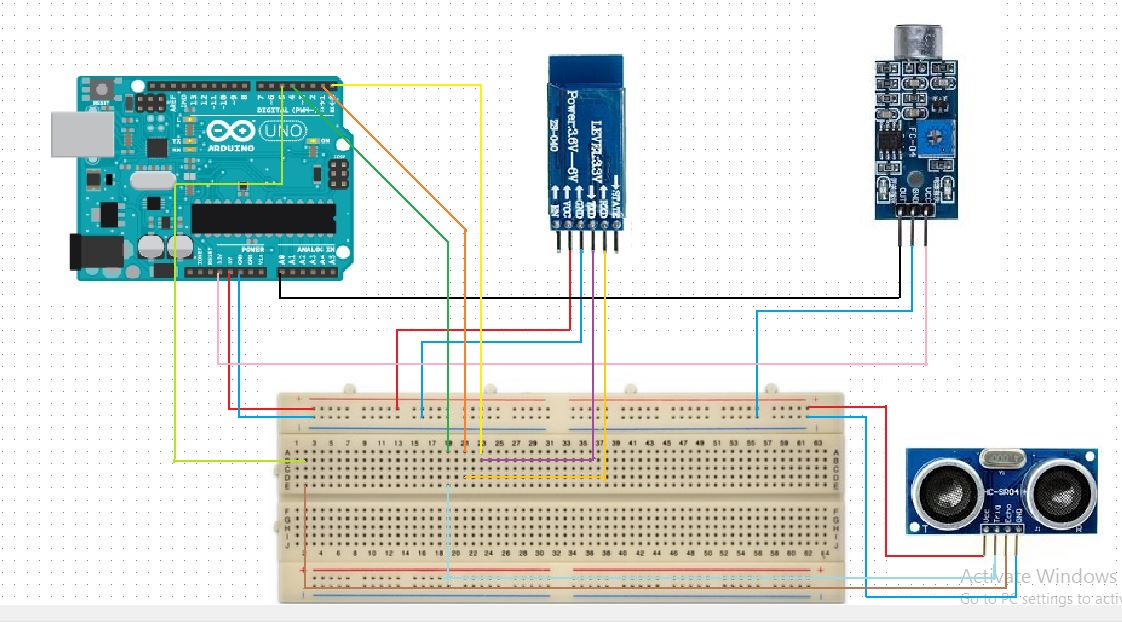
\includegraphics[width=5.7in]{master}}
\caption{Master device architecture .}
\end{figure}
\begin{figure}[h]
\centerline{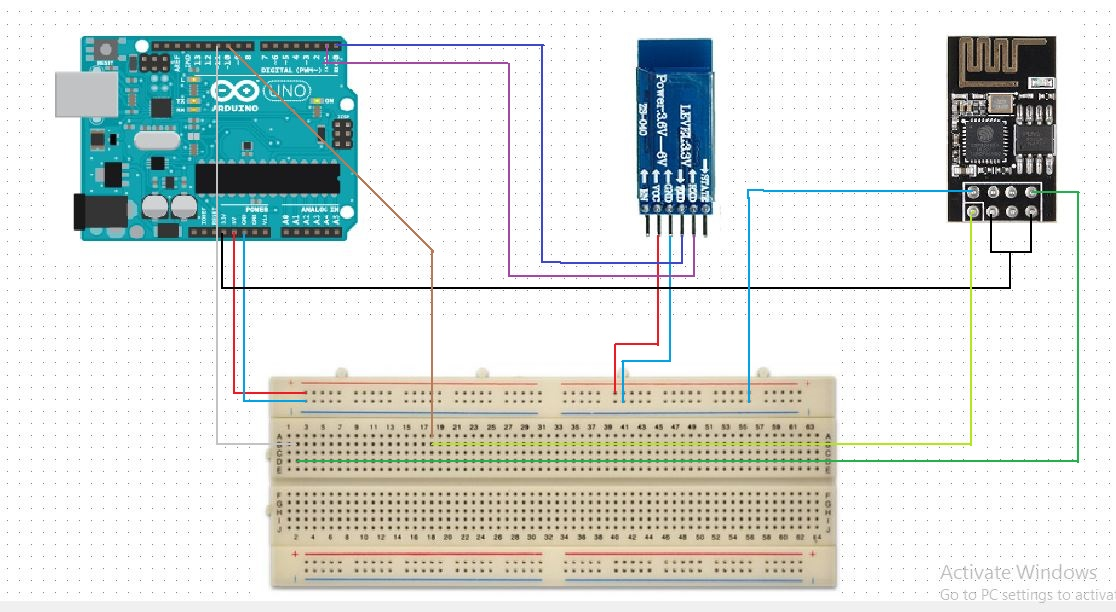
\includegraphics[width=5.7in]{slave}}
\caption{slave device architecture.}
\end{figure}
\section{Implementation}
Our major implementation part begins with the embedding of sensors on the Arduino board and experimenting with them, and the major components are master and slave devices these are explained below
\subsection{Master Device}
The master device consists of one Arduino board, an ultrasonic sensor, a sound sensor, a vibration sensor, a humidity and temperature sensor, smoke sensor and a Bluetooth module HC-05.

\begin{figure}[h]
\centerline{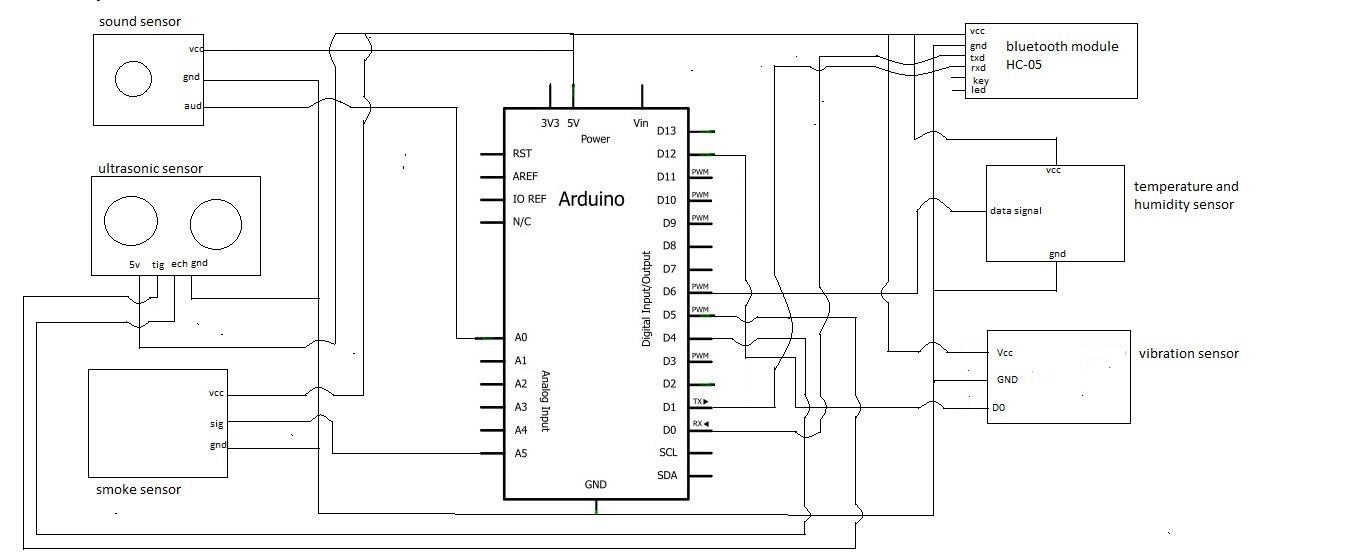
\includegraphics[width=5.7in]{MC}}
\caption{ Master Circuit Diagram.}
\end{figure}
Five sensors and a Bluetooth module is integrated in a single Arduino board for monitoring the health condition of the industrial machines. We can use any set of sensors according to the requirement of the industrial machines. It is basically used to collect the data and transfer to the slave device. The connections in the circuit are as follow.
\subsubsection{Ultrasonic sensor}
The ultrasonic sensor consists of four pins. They are Vcc pin, ground pin, Trigger pin, echo pin.The Vcc pin is connected to +5 volt pin of the Arduino board, the ground pin is connected to the ground pin of the Arduino pin, the Trigger pin is connected to the digital pin 4 of the Arduino board and the echo pin is connected to the digital pin 5 of the Arduino board. The sensor is powered by the Vcc pin with +5 volts. The Trigger pin is an Input pin and is set to HIGH with a +5 volt power and it transmits ultrasonic waves. The ultrasonic waves travels straight until it is blocked by any object then the waves bounces back. The echo pin is an output pin which goes HIGH a period of time until the waves reach back to the sensor. The distance travelled by the wave before it bounce back after blocked by any object is calculated by using the formula

 Distance (D) =1/2*duration*sonic speed [sonic speed=0.034]
 
 \subsubsection{Sound sensor}
 The sound sensor consists of a microphone and three pins. They are Vcc pin, ground pin and OUT pin. The sound sensor has a potentiometer also for adjusting sensitivity threshold selection. The Vcc pin is connected to the +5 volts of the Arduino board, the ground pin is connected to ground of the Arduino board and OUT pin is connected to the analog pin 1 of the Arduino board. The sensor is powered by the Vcc pin with +5 volts. The OUT pin is an Input pin and we set a certain threshold value to the sensor if the sound around the sensor exceeds the threshold value the OUT pin goes to HIGH. The microphone attached to the sensor converts the sound into analog value and you can see the analog value in the serial monitor of the Arduino
IDE.
\subsubsection{SM-420 Vibration sensor}
The vibration sensor consists of a potentiometer and three pins. They are Vcc pin, ground pin and D0 pin. The potentiometer is used for adjusting sensitivity threshold selection. The Vcc pin is connected to the +5 volts of the Arduino board, the ground pin is connected to the ground of the Arduino board and D0 pin is connected to the digital pin 12 of the Arduino board. The sensor is powered with +5 volts. The D0 pin is an input pin when there is vibration the sensor feels the vibration and the D0 pin goes to HIGH, if there is no vibration the D0 pin goes to LOW. The threshold value can be set by using the potentiometer.
\subsubsection{MQ-2 Smoke sensor}
The smoke sensor consists of a potentiometer and three pins. They are Vcc pin, ground pin, signal pin. As smoke sensor can detect a wide range of gases like hydrogen, propane, butane, LPG, alcohol. The potentiometer is adjusted according to the requirement. The Vcc pin is connected +5 volts of the Arduino board, the ground pin is connected the ground of the Arduino board and the signal pin is connected to the analog pin 5 of the Arduino board. The sensor is powered by +5 volts. The signal pin is an input pin and its goes to HIGH when the gas is detected and LOW when there is no gas. The output voltage depends upon the concentration of the gases. The higher the concentration higher the output voltage. The lower the concentration lower the output voltage.
\subsubsection{Humidity and temperature sensor}
Humidity and temperature sensor consists of three pins mounted on a small PCB which includes a surface mounted 10K Ohm pull up resistor for the signal line. The three pins are Vcc pin which is connected to the +5 volts of the Arduino board, ground pin is connected to the ground of the Arduino board and the data signal pin to the digital pin 6 of the Arduino board. The sensor has humidity range of 20-90% RH, humidity accuracy of + or -5% RH, temperature range of 0-50 degrees C and temperature accuracy of + or -2 degree C. The
sensor is powered by +5 volts. The signal data pin is always kept HIGH by a 5 volts power.The sensor detects the relative humidity by the change in the resistance of the two electrodes in the PCB and temperature is detected by the thermistor built in the PCB on the surface of the sensor.
\subsubsection{Bluetooth module HC-05 (Master)}
The Bluetooth module has 6 pins but we use 4 pins only they are Vcc pin, GND pin, TXD pin and RXD pin. The Bluetooth module has a button switch used to set the Bluetooth module into AT mode for configurations. The Bluetooth module can be connected to an Android device or another Bluetooth module. Once Bluetooth module is connected it transfers or receives data for other devices. The Vcc pin is connected to the +5 volts of the Arduino board, the GND pin is connected to the ground of the Arduino board, the TXD pin is
connected to the digital pin 0 of the Arduino board and RXD pin is connected to the digital pin 1 of the Arduino board. The Bluetooth module is powered by the +5 volts. The TXD and RXD pins are used for communication of the data. Once the connection is established between the master device and slave device the data collected from sensors in master device is sent to the slave device.
\subsection{Slave Device}
This device which helps in collecting all the data from the master device and transfer into the cloud platforms 
\begin{figure}[h]
\centerline{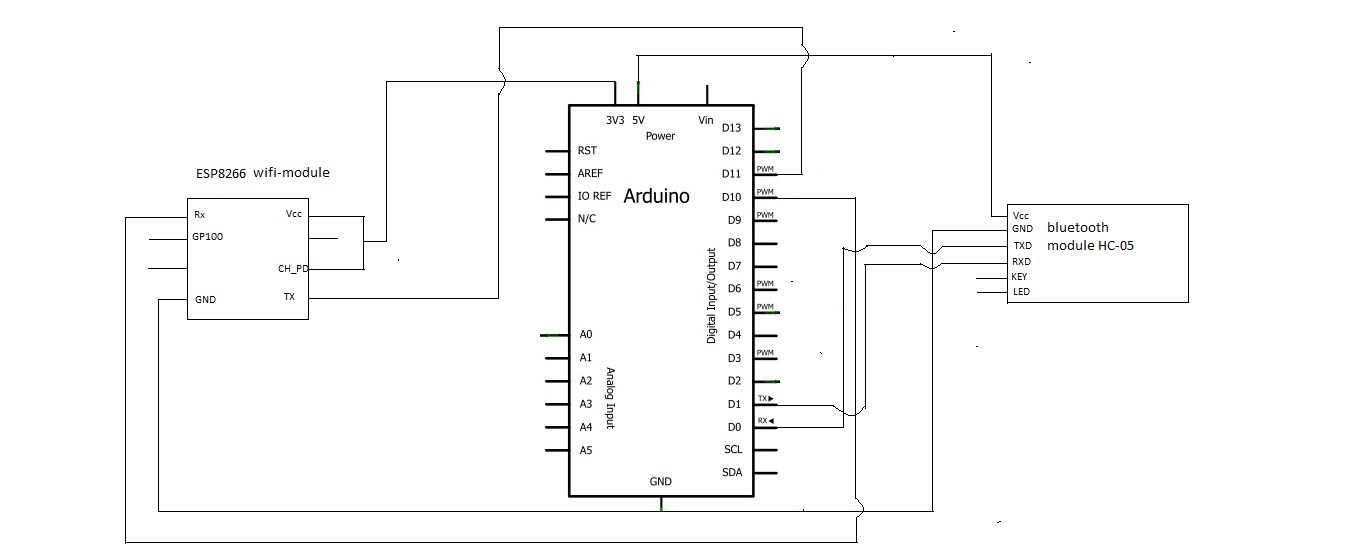
\includegraphics[width=5.7in]{SC}}
\caption{ Slave Circuit Diagram.}
\end{figure}
\subsubsection{Bluetooth module HC-05 (slave)}
The description and connections are same as above. Here the data is received from the master device. The Bluetooth module uses Bluetooth SPP (serial port protocol) for communication.
\subsubsection{ESP8266 Wi-Fi module}
The Wi-Fi module has 8 pins but we use five pins they are Vcc pin, GND pin, TX pin, RX pin and CHPD pin. The Vcc pin and CHPD pin are connected to the +3.3 volts pin of the Arduino board, the GND pin is connected to the ground of the Arduino board, the TX pin is connected to the digital pin 11 of the Arduino board and the RX pin is connected to the digital pin 10 of the Arduino board. The AT commands are used to configure the Wi-Fi module into a router or as access point. Here we are using it as an access point where it is connected to a Wi-Fi router. The data is send to the cloud by the Wi-Fi module.

\subsection{Mode of wireless communication}
Once the testing of sensors is finished we connect both these sensors to one Arduino board. Here we want communicate from one Arduino to another Arduino as here we are using two Bluetooth modules. The AT commands are used to configure them into master and slave Bluetooth. This process is called Master-Slave configuration. For our convenience we name Bluetooth modules Master and Slave Bluetooth modules. The master Bluetooth module is connected with the sensors to one board and slave Bluetooth module to another Arduino board. Once both Bluetooth are connected data is sent or received from one Arduino to another Arduino board.
The Bluetooth module uses the Bluetooth serial port protocol to communicate with other devices such as android devices, other Bluetooth modules etc. The Bluetooth module always reconnects with its previous connected device so the master Bluetooth will always connects with its slave Bluetooth after master-slave configuration. The data is transferred from one Bluetooth module to another Bluetooth module.
\subsection{Storage of data }
The Arduino with slave Bluetooth module is connected to raspberry pi with an USB cable. From raspberry pi we send data to the cloud using python codes. The cloud service we are using here is Think speak. The data received is stored inside the Think speak cloud which stores the data. Then we can analysis the data in the cloud. Once the data from both the sensors is collected and stored we use machine learning to sort the data and use to determine the efficiency of the machine
\section{Testing}
The above set we are going to install inside the AC central room where we check the health condition of the machines by taking inputs from the sensor. By using the inputs we take from the sensor where we will set some threshold value to see that machine is working under good condition. We access the inputs from sensor in cloud by using machine learning.






